\documentclass{article}

\usepackage{hyperref}
\usepackage{amsmath}
\usepackage{graphicx}
\usepackage{subcaption}
\usepackage{epstopdf}
\usepackage{color}

\usepackage{times}
\usepackage{bm}

% Page layout
\hoffset -0in
\voffset -1in
\oddsidemargin 0in
\textheight 9.3in
\textwidth 6.3in

\renewcommand{\arraystretch}{1.3}
\setlength{\parindent}{0pt}
%\setlength{\intextsep}{10pt}
%\pagestyle{empty}

\graphicspath{{figures/}}

\begin{document}
\section*{COMPUTATIONAL METHODS IN MECHANICS: Assignment 6}
Vesa-Ville Hurskainen, 27 Feb 2018\\
\href{https://github.com/VesaVilleHurskainen/cmim2018}{GitHub repository}

\section*{Introduction}
This is a report of the sixth assignment of the course \textit{Computational Methods in Mechanics}. The assignment consists of four tasks, which are as follows:
\begin{enumerate}
	\setlength\itemsep{0pt}
	\item To derive the spatial rotation matrix resulting from the (zxz) Euler angles $\alpha = 45^\circ$, $\beta = 45^\circ$, $\gamma = 45^\circ$.
	\item To derive the (zxz) Euler angles and Euler parameters associated with rotating coordinate frame 1 by angle $\varphi = \pi/6$ about axis $y_0$ of frame 0, assuming that the frames are initially parallel.
	\item To derive the first and second time derivatives of a given matrix function $\mathbf{C}(\bm{q},t)$, assuming $\bm{q}(t)$.
	\item To solve the coordinates of a given mechanism using Newton-Raphson method and given initial values.
\end{enumerate}

\section*{Task 1}
Elemental spatial rotations can be expressed in rotation matrix form as follows:
\begin{equation}
\mathbf{A}_x (\varphi) =
\begin{bmatrix}
	1 & 0 & 0\\
	0 & \cos \varphi & -\sin \varphi \\
	0 & \sin \varphi & \cos \varphi
	\end{bmatrix},
	\quad
	\mathbf{A}_y (\varphi) =
	\begin{bmatrix}
	\cos \varphi & 0 & \sin \varphi\\
	0 & 1 & 0 \\
	-\sin \varphi & 0 & \cos \varphi
	\end{bmatrix},
	\quad
	\mathbf{A}_z (\varphi) =
	\begin{bmatrix}
	\cos \varphi & -\sin \varphi & 0\\
	\sin \varphi & \cos \varphi & 0 \\
	0 & 0 & 1
\end{bmatrix}
\end{equation}
Therefore, the rotation matrix resulting from the zxz-type (extrinsic) Euler angles $\alpha = 45^\circ$, $\beta = 45^\circ$, $\gamma = 45^\circ$ is:
\begin{equation}
\mathbf{A} = \mathbf{A}_z (\gamma) \mathbf{A}_x (\beta) \mathbf{A}_z (\alpha) =
\begin{bmatrix}
	\frac{1}{2} - \frac{1}{\sqrt{8}} & -\frac{1}{2} - \frac{1}{\sqrt{8}} & \frac{1}{2} \\
	\frac{1}{2} + \frac{1}{\sqrt{8}} & -\frac{1}{2} + \frac{1}{\sqrt{8}} & -\frac{1}{2} \\
	\frac{1}{2} & \frac{1}{2} & \frac{1}{\sqrt{2}}
	\end{bmatrix}
	\approx
	\begin{bmatrix}
	0.146 & -0.854 & 0.5 \\
	0.854 & -0.146 & -0.5 \\
	0.5 & 0.5 & 0.707
\end{bmatrix}
\end{equation}

\section*{Task 2}
Assuming that coordinate frame 0 is coincident with the global frame (i.e., extrinsic rotations are performed about the axes of frame 0), rotation by $\varphi = \frac{\pi}{6}$ rad about axis $y_0$ can be performed using zxz-type Euler angles via the following algorithm:
\begin{enumerate}
	\setlength\itemsep{0pt}
	\item Rotate frame 1 about $z_0$ by $-\frac{\pi}{2}$ rad, so that $y_1$ coincides with $x_0$.
	\item Rotate frame 1 about $x_0$ by $\frac{\pi}{6}$ rad, accomplishing the desired rotation.
	\item Rotate frame 1 about $z_0$ by $\frac{\pi}{2}$ rad, "undoing" the first rotation.
\end{enumerate}
Therefore, the Euler angles for this rotation are $\alpha = -\frac{\pi}{2}$, $\beta = \frac{\pi}{6}$, $\gamma = \frac{\pi}{2}$.\\

To get the corresponding Euler parameters, knowing that rotation axis
$\renewcommand{\arraystretch}{1}\bm{k} = \begin{bmatrix} 0 & 1 & 0 \end{bmatrix}^\text{T}$, 
we can calculate: 
\begin{equation}
\bm{p} =
\begin{bmatrix}
	\cos \frac{\varphi}{2} & k_x \sin \frac{\varphi}{2} & k_y \sin \frac{\varphi}{2} & k_z \sin \frac{\varphi}{2}
\end{bmatrix}^\text{T}
=
\begin{bmatrix}
	\frac{1}{4}(\sqrt{6} + \sqrt{2}) & 0 & \frac{1}{4}(\sqrt{6} - \sqrt{2}) & 0
\end{bmatrix}^\text{T}
\end{equation}
Constructing rotation matrices using these methods, we can see that both result in the elemental rotation matrix:
\begin{equation}
\mathbf{A} = \mathbf{A}_y (\frac{\pi}{6}) =
\begin{bmatrix}
	\frac{\sqrt{3}}{2} & 0 & \frac{1}{2}\\
	0 & 1 & 0 \\
	-\frac{1}{2} & 0 & \frac{\sqrt{3}}{2}
\end{bmatrix}
\end{equation}

\clearpage
\section*{Task 3}
Matrix $\mathbf{C}$ is defined as follows:
\begin{equation}
\mathbf{C} = 
\begin{bmatrix}
	x^2 + y + \sqrt{z} + \sin \varphi_1 \\
	xy + xz + y \sin \varphi_3 + t^3 \\
	\sin \varphi_2 + x^\frac{3}{2} + t
\end{bmatrix}
\end{equation}
Assuming that vector
$\renewcommand{\arraystretch}{1}\bm{q} = \begin{bmatrix} x & y & z & \varphi_1 & \varphi_2 & \varphi_3 \end{bmatrix}^\text{T}$
is a function of time and differentiating by hand, we get:
\begin{equation}
\dot{\mathbf{C}} = 
\begin{bmatrix}
	2 x \dot{x} + \dot{y} + \frac{\dot{z}}{2 \sqrt{z}} + \dot{\varphi}_1 \cos \varphi_1 \\
	\dot{x} (y + z) + x (\dot{y} + \dot{z}) + \dot{y} \sin \varphi_3 + y \dot{\varphi}_3 \cos \varphi_3 + 3 t^2\\
	\dot{\varphi}_2 \cos \varphi_2 + \frac{3}{2} \dot{x} \sqrt{x} + 1
\end{bmatrix}
\end{equation}
\begin{equation}
\ddot{\mathbf{C}} = 
\begin{bmatrix}
	2 \ddot{x} x + 2 \dot{x}^2 + \ddot{y} + \frac{\ddot{z}}{2 \sqrt{z}} - \frac{\dot{z}^2}{4 \sqrt{z^3}} + \ddot{\varphi}_1 \cos \varphi_1 - \dot{\varphi}_1^2 \sin \varphi_1 \\
	\ddot{x} (y + z) + 2 \dot{x} (\dot{y} + \dot{z}) + x (\ddot{y} + \ddot{z}) + (\ddot{y} - y \dot{\varphi}_3^2) \sin \varphi_3 + (2 \dot{y} \dot{\varphi}_3 + y \ddot{\varphi}_3) \cos \varphi_3 + 6 t \\
	\ddot{\varphi}_2 \cos \varphi_2 - \dot{\varphi}_2^2 \sin \varphi_2 + \frac{3}{2} \ddot{x} \sqrt{x} + \frac{3 \dot{x}^2}{4 \sqrt{x}}
\end{bmatrix}
\end{equation}
Symbolic differentiation in MATLAB produces identical results.

\section*{Task 4}
Using Figure~\ref*{fig:system}, we can derive geometrical equations to describe the system's position. For example:
\begin{equation}
\begin{aligned}
h &= r \sin \varphi \\
c &= r \cos \varphi
\end{aligned}
\end{equation}
With the parameters $h = 4$ m and $c = 3$ m, solving these equations by hand is trivial. However, as per instructions, the equations were solved numerically using the Newton-Raphson method, using the initial values $r^0 = 4$ m and $\varphi^0 = 4$ m. This was performed using the script \texttt{task4.m} and the function \texttt{newtonRaphson.m}, which was created for the previous assignment. With both approaches, the result is $r = 5$ m, $\varphi = \tan^{-1} \frac{4}{3} \approx 0.927$ rad.

\begin{figure}[h]
	\centering
	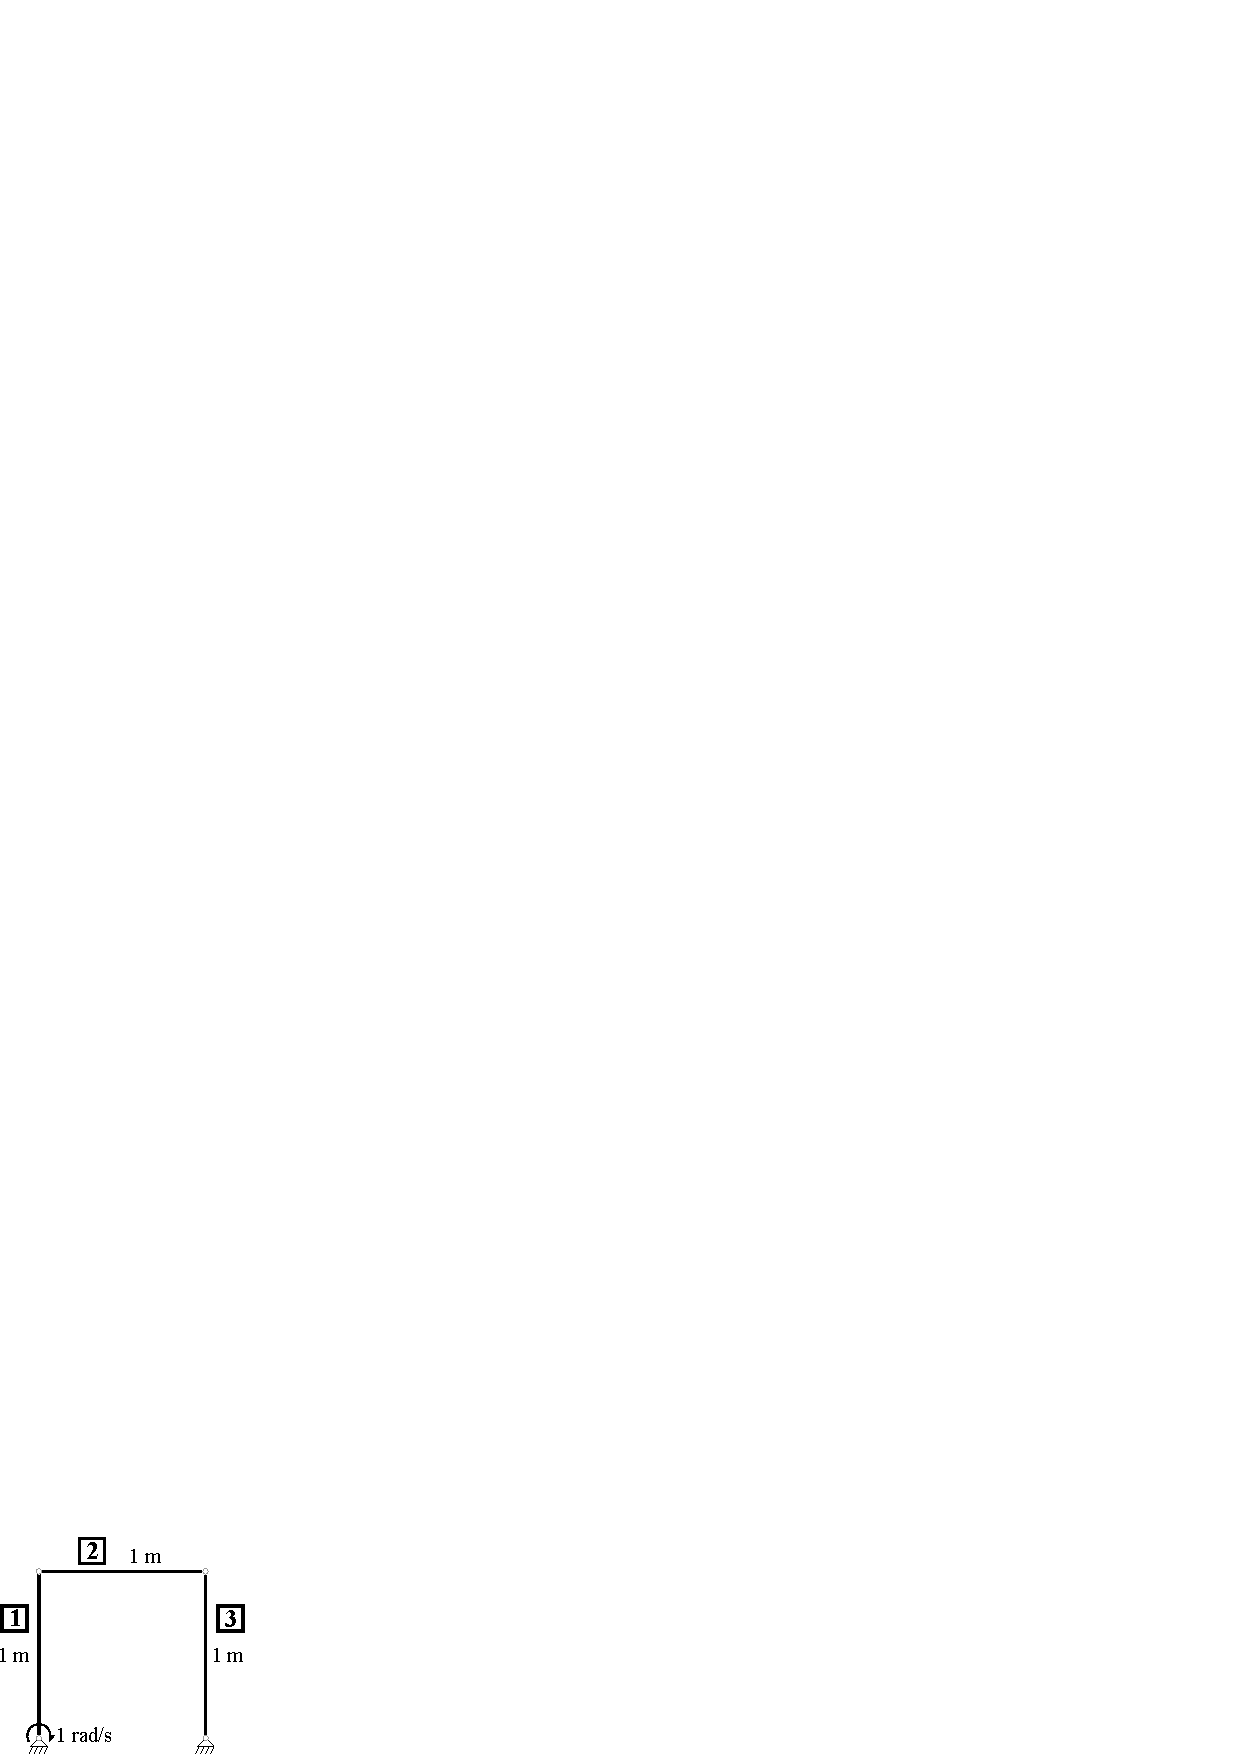
\includegraphics[width=0.4\textwidth]{system.png}
	\caption{System geometry (Orzechowski, 2018).}
	\label{fig:system}
\end{figure}
\end{document}